\documentclass{beamer}
\usepackage[english]{babel}
\usepackage[latin1]{inputenc}
\usepackage{enumerate}
\usepackage{amsmath}
\usepackage{graphicx}
\usepackage{subfigure}
\usetheme{Warsaw}

\AtBeginSection[]
{
  \begin{frame}
    \frametitle{Table of Contents}
    \tableofcontents[currentsection]
  \end{frame}
}

\begin{document}
\title{Prediction using Bayesian Networks}
\author{Inge Becht}
\institute{University of Amsterdam}
\date{\today}


\begin{frame}
  \titlepage
\end{frame}

\begin{frame}{Subject}
    \begin{itemize}
        \item{
                Will I be moving to a new appartment?
            }
        \item{ Considering a 2 year span}
        \item{ Some more probable events and some less probable}
    \end{itemize}
\end{frame}


\begin{frame}{Creating the network}
    \begin{itemize}
        \item What causes me to move?
            \begin{itemize}
                \item Change in income
                    \begin{itemize}
                        \item lower
                        \item higher
                    \end{itemize}
                \item House gets unlivable
                \item Noisy neighbours
                \item etc.
            \end{itemize}
        \item And what causes these things?
    \end{itemize}
\end{frame}


\begin{frame}{Modelling problems}
    \begin{itemize}
        \item How to represent money gain, money loss or money income that stays
            the same?
            \begin{itemize}
                \item Creating multiple boolean nodes that are dependent of
                    eachother 
                \item Creating a node with multiple values(not boolean)
            \end{itemize}
        \item Can noisy OR be implemented?
            \begin{itemize}
                \item Probably not all the time!
            \end{itemize}
    \end{itemize}
\end{frame}

\begin{frame}{Models compared}
    Con: we now have $2^3$ probabilities in regards to moving, from which some aren't even
    possible combinations.
    \begin{figure}[h!]
  \centering
    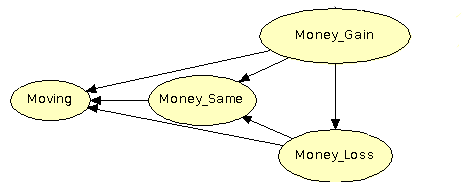
\includegraphics[width=0.7\textwidth]{booleanMoney.png}
  \caption{Using booleans to represent money.}
\end{figure}
\end{frame}


\begin{frame}{Models compared (2)}
    Now only 3 probabilities to consider\\
    Con: How can Noisy OR be used?
\begin{figure}[h!]
  \centering
    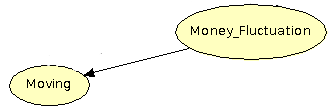
\includegraphics[width=0.5\textwidth]{3ValueMoney.png}
  \caption{Money fluctuation represented as 3 nodes.}
\end{figure}
\end{frame}


\begin{frame}{The final network: Moneygain}
\begin{figure}[h!]
  \centering
    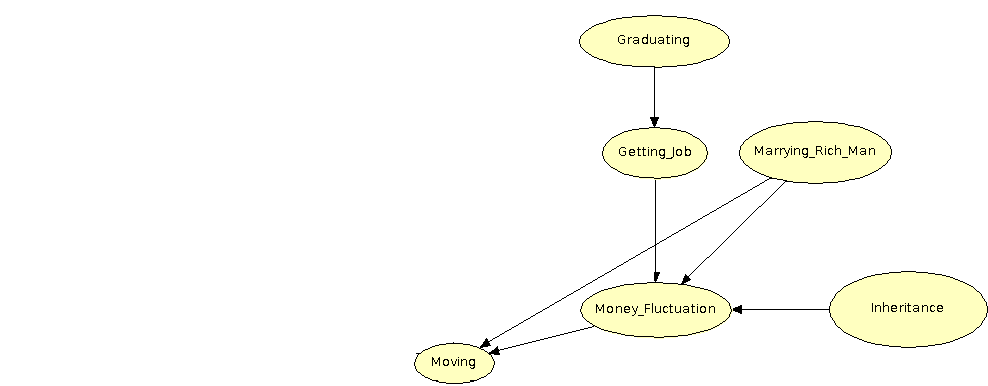
\includegraphics[width=1.1\textwidth]{network1.png}
  \caption{Money dependencies}
\end{figure}
\end{frame}

\begin{frame}{The tables(1)}
    \begin{table}
\centering
\makebox[0pt][c]{\parbox{1.2\textwidth}{%
    \begin{minipage}[b]{0.5\hsize}\centering
        \begin{tabular}{ | c | c |}
           \hline
           & $\mu{(Graduating)}$ \\ \hline
           1 & 0.8 \\ \hline
           0 & 0.2 \\ \hline
        \end{tabular}
        \caption{Chance of graduating}
        \label{tab:singlebest}
    \end{minipage}
   \hfill
    \begin{minipage}[b]{0.5\hsize}\centering
        \begin{tabular}{ | c | c |}
           \hline
           & $\mu(Marrying\_rich\_man)$ \\ \hline
           1 & 0.01\\ \hline
           0 & 0.99 \\ \hline
        \end{tabular}
        \caption{Chance of marrying rich man}
        \label{tab:twobest}
    \end{minipage}
    \hfill
}}
\end{table}
\end{frame}


\begin{frame}{The tables(2)}
    \begin{table}
\centering
\makebox[0pt][c]{\parbox{1.2\textwidth}{%
    \begin{minipage}[b]{0.5\hsize}\centering
        \begin{tabular}{ | c | c |}
           \hline
           & $\mu(Inheritance)$ \\ \hline
           1 & 0.1 \\ \hline
           0 & 0.9 \\ \hline
        \end{tabular}
        \caption{Chance of inheritance}
        \label{tab:threebest}
    \end{minipage}%
   \hfill
    \begin{minipage}[b]{0.5\hsize}\centering
        \begin{tabular}{ | c | cc|}
           \hline
           Graduating  & $\mu{(Job)}$  &$\mu(\neg Job)$\\ \hline
           1 & 0.8 & 0.2 \\ \hline
           0 & 0.2 & 0.8\\ \hline
        \end{tabular}
        \caption{Chance of graduating}
    \end{minipage}
    \hfill
}}
\end{table}
\end{frame}

\begin{frame}{The tables(3)}
\begin{centering}
\begin{table}
\begin{tabular}{|lll|lll|}
  \hline
  M & I & G & $\mu(more)$ & $\mu(same)$  & $\mu(less)$  \\ \hline
  0 & 0 & 0 &   0.1 & 0.6 & 0.3 \\
  0 & 0 & 1  &  0.8    & 0.2 & 0       \\ 
  0 & 1 & 0  &  0.3    & 0.4 & 0.3     \\
  1 & 0 & 0  &  0.9    & 0.1 & 0     \\                     
  0 & 1 & 1  &  0.8    & 0.1 & 0.1\\       
  1 & 0 & 1  &  1        & 0 & 0\\   
  1 & 1 & 0  &  0.9    & 0.1 & 0\\         
  1 & 1 & 1  &  0.99   & 0.01 & 0 \\
  \hline
\end{tabular}
\caption{Probability of money fluctuation}
\end{table}
\end{centering}
\end{frame}


\begin{frame}{The final network: Noisiness}
\begin{figure}[h!]
  \centering
    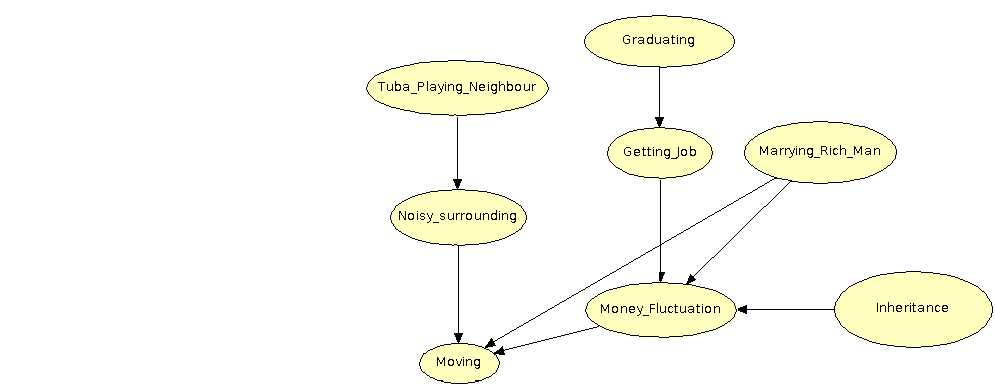
\includegraphics[width=1.1\textwidth]{network2.png}
  \caption{Noisiness dependencies}
\end{figure}
\end{frame}


\begin{frame}{The tables}
    \begin{table}
\centering
\makebox[0pt][c]{\parbox{1.2\textwidth}{%
    \begin{minipage}[b]{0.5\hsize}\centering
        \begin{tabular}{ | c | c |}
           \hline
           & $\mu(Tuba\_neighbour)$ \\ \hline
           1 & 0.02 \\ \hline
           0 & 0.98 \\ \hline
        \end{tabular}
        \caption{Chance of tuba playing neighbour}
        \label{tab:threebest}
    \end{minipage}%
   \hfill
    \begin{minipage}[b]{0.5\hsize}\centering
        \begin{tabular}{ | c | cc|}
           \hline
           Tuba  & $\mu{(Noise)}$  &$\mu(\neg Noise)$\\ \hline
           1 & 0.98 & 0.02 \\ \hline
           0 & 0.5 & 0.5\\ \hline
        \end{tabular}
        \caption{Chance of noise}
    \end{minipage}
    \hfill
}}
\end{table}
\end{frame}

\begin{frame}{The final network: Unlivability}
\begin{figure}[h!]
  \centering
    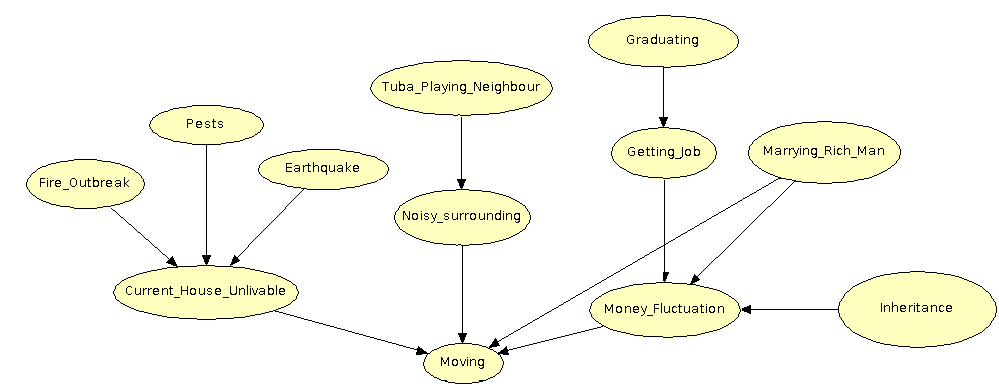
\includegraphics[width=1.1\textwidth]{network3.png}
  \caption{Unlivable dependencies}
\end{figure}
\end{frame}

\begin{frame}{The tables}
    \begin{table}
\centering
\makebox[0pt][c]{\parbox{1.2\textwidth}{%
    \begin{minipage}[b]{0.3\hsize}\centering
        \begin{tabular}{ | c | c |}
           \hline
           & $\mu{(Fire)}$ \\ \hline
           1 & 0.01 \\ \hline
           0 & 0.99 \\ \hline
        \end{tabular}
        \caption{Chance of fire}
        \label{tab:singlebest}
    \end{minipage}
   \hfill
    \begin{minipage}[b]{0.3\hsize}\centering
        \begin{tabular}{ | c | c |}
           \hline
           & $\mu(pest)$ \\ \hline
           1 & 0.2\\ \hline
           0 & 0.8 \\ \hline
        \end{tabular}
        \caption{Chance of pests}
        \label{tab:twobest}
    \end{minipage}
    \hfill
    \begin{minipage}[b]{0.3\hsize}\centering
        \begin{tabular}{ | c | c |}
           \hline
           & $\mu(Earthquake)$ \\ \hline
           1 & 0.3\\ \hline
           0 & 0.7 \\ \hline
        \end{tabular}
        \caption{Chance of Earthquake}
        \label{tab:twobest}
    \end{minipage}
}}
\end{table}
\end{frame}

\begin{frame}{Noisy OR}
  \begin{itemize}
      \item Not all elements are considered (More variables possible when
          considering money gain)
      \item How to implement noisy OR in case of 3 possible values instead of
          boolean?
    \item Using noisy OR to indicate house livability seems to work very well
  \end{itemize}
\end{frame}

\begin{frame}{noisy OR implemented}
E = Earthquake, P = Pest, F = Fire, U = Unlivable conditions\\
\hspace{5 mm}
\begin{centering}
\begin{table}
\begin{tabular}{|lll|ll|}
  \hline
  E & P & F & $\mu(U)$ & $\mu(\neg U)$   \\ \hline
  0 & 0 & 0 & 0 & 1 \\
  0 & 0 & 1  &  $0.6$       & $0.4$       \\ 
  0 & 1 & 0  &  $0.8$       & $0.2$       \\
  1 & 0 & 0  &  $0.001$     & $0.999$     \\                     
  0 & 1 & 1  &  $0.92$      & $0.4 * 0.2 =0.08$\\       
  1 & 0 & 1  &  $0.6004$    & $0.999 * 0.4 = 0.3996$\\   
  1 & 1 & 0  &  $0.8002$    & $0.999 * 0.2 = 0.1998$\\         
  1 & 1 & 1  &  $0.92008$   & $0.4 * 0.2 * 0.999 = 0.07992$ \\
  \hline
\end{tabular}
\caption{Probability of Unlivable conditions arising}
\end{table}
\end{centering}
\end{frame} 

\begin{frame}{Probability of moving}
    \begin{itemize}
        \item {probability of moving is dependent of money fluctuation,
            noisiness of surroundings, livability of house and if I will be
        getting married}
        \item{24 different combinations of events}
        \item{Problematic pairs like Marrying rich man and Low income occur}
    \end{itemize}
\end{frame}

\begin{frame}{The table}
\begin{centering}
\small
\begin{table}
\begin{tabular}{|llll|ll|}
  \hline
  Marrying & Unlivable & Noisy & Money &  $\mu(Moving)$ & $\mu(\neg Moving)$   \\ \hline
  0 & 0 & 0 & L & 0.7 & 0.3 \\
  0 & 0 & 0 & S & 0 & 1 \\
  0 & 0 & 0 & H & 0.7& 0.3   \\
  0 & 0 & 1 & L & 0.5  & 0.5  \\ 
  0 & 0 & 1 & S & 0.1  & 0.9  \\ 
  0 & 0 & 1 & H & 0.7  & 0.3   \\ 
  0 & 1 & 0 & L & 0.8  & 0.2  \\ 
  0 & 1 & 0 & S & 0.85  & 0.15  \\ 
  0 & 1 & 0 & H & 0.9  &  0.1  \\ 
  \dots  &\dots   &\dots   &\dots   & \dots     &\dots \\
  1 & 0 & 1 & H & 0.9  & 0.1  \\ 
  1 & 1 & 0 & L & 0.9  & 0.1  \\ 
  1 & 1 & 0 & S & 0.95  & 0.05   \\ 
  1 & 1 & 0 & H & 0.95  & 0.05  \\ 
  1 & 1 & 1 & L & 0.9  & 0.1  \\ 
  1 & 1 & 1 & S & 0.99  & 0.01  \\ 
  1 & 1 & 1 & H & 1  & 0   \\ 
  \hline
\end{tabular}
\end{table}
\end{centering}
\end{frame}


\begin{frame}{Chance of moving}
    \begin{itemize}
        \item Chance of moving: 54.6\\
        \item Seems somewhat low given the probability distribution
                    \begin{itemize}
                    \item Only 57 percent chance of earning more
                    \item Most of the nodes are biased towards reasons to move
                    \item But are very small chances of happening

                    \end{itemize}
                \item More nodes (that are more relevant) could give a more accurate result of moving
            probability
    \end{itemize}
\end{frame}

\begin{frame}{Other probabilities}
    \begin{itemize}
        \item Chance of moving given tuba playing neighbours and earning more:
            73.61\\
        \item Chance of moving given pests and earning the same: 56.63
        \item Chance of getting a job given moving and earning the same: 40.82
            \begin{itemize}
                \item  Seems a bit much...
            \end{itemize}
        \item Chance of graduating when not getting a job: 50
    \end{itemize}
\end{frame}
\end{document}
